%%%%%%%%%%%%%%%%%%%%%%%%%%%%%%%%%%%%%%%%%%%%%%%%%%%%%%%%%%%%%%%%%%%%%%%%%%%%%%%%%%%%%%%%%%%%%%%%%%%%%%%%
%% Template para o artigo do evento da SOBRAC 2018
%% Desenvolvido por Prof. William D'Andrea Fonseca - Eng. Acústica UFSM
%% Versão de 13/04/2018
%%%%%%%%%%%%%%%%%%%%%%%%%%%%%%%%%%%%%%%%%%%%%%%%%%%%%%%%%%%%%%%%%%%%%%%%%%%%%%%%%%%%%%%%%%%%%%%%%%%%%%%%
\documentclass[12pt, a4paper, oneside, onecolumn] {article}%
%%%%%%%%%%%%%%%%%%%%%%%%%%%%%%%%%%%%%%%%%%%%%%%%%%%%
%%% Linguagem e entrada
\usepackage[utf8]{inputenc} 
\usepackage[english,brazil]{babel}
\usepackage{mathptmx} % Times
%%%%%%%%%%%%%%%%%%%%%%%%%%%%%%%%%%%%%%%%%%%%%%%%%%%%%%%%%%%%%%%%%%%%%%%%%
\usepackage{Sobrac2018} %%% Configurações básicas do template
%%%%%%%%%%%%%%%%%%%%%%%%%%%%%%%%%%%%%%%%%%%%%%%%%%%%%%%%%%%%%%%%%%%%%%%%%
\usepackage{Will} %%% Pacote com configurações adicionais e opcionais
%%%%%%%%%%%%%%%%%%%%%%%%%%%%%%%%%%%%%%%%%%%%%%%%%%%%%%%%%%%%%%%%%%%%%%%%%%%%%%%%%%%%%%%%%%%%%%%%%%%%%%%%
% PDF Metadata
\hypersetup{pdftex,
            pdfauthor={ Coloque os autores aqui },
            pdftitle={ Coloque o título aqui },
            pdfsubject={ Coloque o assunto do artigo aqui },
            pdfkeywords={ Colocar palavras-chave aqui },
            pdfproducer={Sobrac 2018},
            pdfcreator={Latex with PDFLatex},
						pdfstartview={FitH}}
%%%%%%%%%%%%%%%%%%%%%%%%%%%%%%%%%%%%%%%%%%%%%%%%%%%%%%%%%%%%%%%%%%%%%%%%%%%%%%%%%%%%%%%%%%%%%%%%%%%%%%%%			
%\usepackage{lineno} \linenumbers %%% Ative para numerar as linhas
%%%%%%%%%%%%%%%%%%%%%%%%%%%%%%%%%%%%%%%%%%%%%%%%%%%%%%%%%%%%%%%%%%%%%%%%%%%%%%%%%%%%%%%%%%%%%%%%%%%%%%%%
% Comandos para revisão duplo-cego
\newcommand{\brev}[1]{#1} % Utilize esse comando para revelar detalhes de identificação (brev = blind review)
%\newcommand{\brev}[1]{\textit{AAA}} % Utilize esse comando para OMITIR detalhes de identificação
%%%%%%%%%%%%%%%%%%%%%%%%%%%%%%%%%%%%%%%%%%%%%%%%%%%%%%%%%%%%%%%%%%%%%%%%%%%%%%%%%%%%%%%%%%%%%%%%%%%%%%%%
\begin{document} % Início do conteúdo
%%%%%%%%%%%%%%%%%%%%%%%%%%%%%%%%%%%%%%%%%%%%%%%%%%%%%%%%%%%%%%%%%%%%%%%%%%%%%%%%%%%%%%%%%%%%%%%%%%%%%%%%
\begin{center} 
\Cabecalho
%%%%%%%%%%%%%%%%%%%%%%%%%%%%%%%%%%%%%%%%%%%%%%%%%%%%%%%%%%%%%%%%%%%%%
%%%%%%%%%%%%%%%%%%%%%%%%%%%%%%%%%%%%%%%%%%%%%%%%%%%%%%%%%%%%%%%%%%%%%
{\fontsize{14}{18}\selectfont \bfseries \uppercase{
%%%%%%%%%%%%%%%%%%%%%%%%%%%%%%%%%%%%%%%%%%%%%%%%%%%%%%%%%%%%%%%%%%%%%%%%%%%%%%%%%%%%%%%%%%%%%%%%%%%%%%%%
%%%%%%%%%%%%%%%%%%%%%%%%%%%%%%%%%%%%%%%%%%%%%%%%%%%%%%%%%%%%%%%%%%%%%%%%%%%%%%%%%%%%%%%%%%%%%%%%%%%%%%%%
Título do artigo
%%%%%%%%%%%%%%%%%%%%%%%%%%%%%%%%%%%%%%%%%%%%%%%%%%%%%%%%%%%%%%%%%%%%%%%%%%%%%%%%%%%%%%%%%%%%%%%%%%%%%%%%
%%%%%%%%%%%%%%%%%%%%%%%%%%%%%%%%%%%%%%%%%%%%%%%%%%%%%%%%%%%%%%%%%%%%%%%%%%%%%%%%%%%%%%%%%%%%%%%%%%%%%%%%
}\\[18pt]\par} {\fontsize{12}{15}\selectfont 
%%%%%%%%%%%%%%%%%%%%%%%%%%%%%%%%%%%%%%%%%%%%%%%%%%%%%%%%%%%%%%%%%%%%%%%%%%%%%%%%%%%%%%%%%%%%%%%%%%%%%%%%
%%%%%%%%%%%%%%%%%%%%%%%%%%%%%%%%%%%%%%%%%%%%%%%%%%%%%%%%%%%%%%%%%%%%%%%%%%%%%%%%%%%%%%%%%%%%%%%%%%%%%%%%
\brev{Sobrenome, Prenomes$^{1}$; Sobrenome, Prenomes$^{2}$}
%Sobrenome, Prenomes$^{3}$; Sobrenome, Prenomes$^{4}$
%%%%%%%%%%%%%%%%%%%%%%%%%%%%%%%%%%%%%%%%%%%%%%%%%%%%%%%%%%%%%%%%%%%%%%%%%%%%%%%%%%%%%%%%%%%%%%%%%%%%%%%%
%%%%%%%%%%%%%%%%%%%%%%%%%%%%%%%%%%%%%%%%%%%%%%%%%%%%%%%%%%%%%%%%%%%%%%%%%%%%%%%%%%%%%%%%%%%%%%%%%%%%%%%%
\\[14pt]\par}
%%%%%%%%%%%%%%%%%%%%%%%%%%%%%%%%%%%%%%%%%%%%%%%%%%%%%%%%%%%%%%%%%%%%%
\brev{
{\fontsize{10}{13} \selectfont (1)\, Instituição, endereço, e-mail. \\[2pt]\par}
{\fontsize{10}{13} \selectfont (2)\, Instituição, endereço, e-mail. \\[2pt]\par}
}
\end{center} \vspace{16pt}
%%%%%%%%%%%%%%%%%%%%%%%%%%%%%%%%%%%%%%%%%%%%%%%%%%%%%%%%%%%%%%%%%%%%%%%%%%%%%%%%%%%%%%%%%%%%%%%%%%%%%%%%
{\fontsize{12}{14} \selectfont \bfseries \uppercase{Resumo}}\\[6pt]
{\fontsize{11}{14.5} \selectfont 
%%%%%%%%%%%%%%%%%%%%%%%%%%%%%%%%%%%%%%%%%%%%%%%%%%%%%%%%%%%%%%%%%%%%%%%%%%%%%%%%%%%%%%%%%%%%%%%%%%%%%%%%
%%% Resumo %%%%%%%%%%%%%%%%%%%%%%%%%%%%%%%%%%%%%%%%%%%%%%%%%%%%%%%%%%%%%%%%%%%%%
Este artigo-modelo apresenta as instruções para apresentação de artigos para o XXVIII Encontro da Sociedade Brasileira de Acústica (Sobrac 2018) que será realizado entre os dias 3 e 5 de outubro de 2018 na cidade de Porto Alegre, RS. Os artigos completos a serem submetidos deverão ter, no máximo, 10 páginas. Os resumos deverão possuir no máximo 300 palavras, sem a presença de equações, figuras, tabelas ou referências. Os artigos submetidos serão analisados buscando conformidade com as sessões temáticas definidas. 
%%%%%%%%%%%%%%%%%%%%%%%%%%%%%%%%%%%%%%%%%%%%%%%%%%%%%%%%%%%%%%%%%%%%%%%%%%%%%%%%
}\\[6pt]
%
%%%% Plavras-chave
\textbf{Palavras-chave:}{\fontsize{11}{12}\selectfont 
 artigos, acústica, referências.
}\\[18pt]
%%%%%%%%%%%%%%%%%%%%%%%%%%%%%%%%%%%%%%%%%%%%%%%%%%%%%%%%%%%%%%%%%%%%%%%%%%%%%%%%%%%%%%%%%%%%%%%%%%%%%%%%
%%% Abstract %%%%%%%%%%%%%%%%%%%%%%%%%%%%%%%%%%%%%%%%%%%%%%%%%%%%%%%%%%%%%%%%%%%
\txtEN % Seleciona inglês
{\fontsize{12}{12} \selectfont \bfseries \uppercase{Abstract}}\\[6pt]
{\fontsize{11}{14.5} \selectfont 
%%% Abstract %%%%%%%%%%%%%%%%%%%%%%%%%%%%%%%%%%%%%%%%%%%%%%%%%%%%%%%%%%%%%%%%%%%%%
This article-template shows the instructions for submitting papers to the XXVIII Meeting of the Brazilian Society of Acoustics (Sobrac 2018) that will be held in Porto Alegre, RS, Brazil, from the 3\supe{rd} to 5\supe{th} October 2018. The full paper should not exceed 10 pages. Abstracts must have 300 words maximum, with no equations, figures, tables nor references. Submitted papers are going to be analyzed according to the subject of the technical sessions.
%%%%%%%%%%%%%%%%%%%%%%%%%%%%%%%%%%%%%%%%%%%%%%%%%%%%%%%%%%%%%%%%%%%%%%%%%%%%%%%%
}\\[6pt]
%
%%%% Keywords
\textbf{Keywords:}{\fontsize{11}{12}\selectfont
 papers, acoustics, references.
}\\[2pt]
%%%%%%%%%%%%%%%%%%%%%%%%%%%%%%%%%%%%%%%%%%%%%%%%%%%%%%%%%%%%%%%%%%%%%%%%%%%%%%%%%%%%%%%%%%%%%%%%%%%%%%%%
%%%%%%%%%%%%%%%%%%%%%%%%%%%%%%%%%%%%%%%%%%%%%%%%%%%%%%%%%%%%%%%%%%%%%%%%%%%%%%%%%%%%%%%%%%%%%%%%%%%%%%%%

%%% COnteúdo do artigo

%%% Artigo %%%%%%%%%%%%%%%%%%%%%%%%%%%%%%%%%%%%%%%%%%%%%%%%%%%%%%%%%%%%%%%%%%%%%
\section{Introdução}

É com satisfação que apresentamos este texto para que os autores possam apresentar os artigos de forma padronizada. Isto facilitará muito o trabalho de revisão e diagramação, proporcionando uma uniformidade de texto para os artigos completos, de acordo com a linha temática específica. Neste modelo são apresentadas as principais diretrizes para a elaboração do artigo completo no que diz respeito à apresentação gráfica, à estrutura e ao procedimento para a submissão dos artigos. Este documento já possui a formatação de estilos personalizados para a elaboração do texto. O autor pode, portanto, utilizar este arquivo como modelo para esta finalidade. Serão disponibilizados modelos (\textit{templates}) em Ms Word (.docx) e \LaTeX\xspace (.tex).

O texto completo, até as referências, deverá estar em espaçamento simples entre linhas, tipografia Times New Roman tamanho 12~pts e parágrafo com espaçamento de 0 pts antes e 18~pts depois. É de prática comum a escrita de artigos científicos no impessoal, logo recomenda-se essa prática. Além disso, serão aceitos em língua culta portuguesa, inglesa e espanhola (utilizando a linguagem culta). Palavras estrangeiras deverão ser grafadas em itálico (por exemplo, como em \textit{proceedings}). Os títulos de seções deverão ser apresentados em letras maiúsculas e em negrito, as subseções deverão se também em negrito, porém, com apenas a primeira letra em maiúsculo.  Evite o uso de subseções com mais de três níveis, para isso, busque usar um sistema de listas. 

%%%%%%%%%%%%%%%%%%%%%%%%%%%%%%%%%%%%%%%%%%%%%%%%%%%%%%%%%%%%%%%%%%%%%%%%%%%%%%%%%%%%%%%%%%%%%%%%%%%%%%%%
%%%%%%%%%%%%%%%%%%%%%%%%%%%%%%%%%%%%%%%%%%%%%%%%%%%%%%%%%%%%%%%%%%%%%%%%%%%%%%%%%%%%%%%%%%%%%%%%%%%%%%%%
\setlength\headheight{0pt}
\section{Apresentação gráfica}

Sempre coloque texto em seções e subseções, não as deixe órfãs.

%%%%%%%%%%%%%%%%%%%%%%%%%%%%%%%%%%%%%%%%%%%%%%%%%%%%%%%%%%%%%%%%%%%%%%%%%%%%%%%%%%%%%%%%%%%%%%%%%%%%%%%%
\subsection{Número de páginas}

O trabalho completo deve conter no máximo 10 páginas, não sendo admitido exceder, sob pena de ser excluído da avaliação pelo comitê de revisores. Como forma de otimizar ao máximo o conteúdo de cada página, as figuras podem devem ser apresentadas ao longo do corpo do texto.


%%%%%%%%%%%%%%%%%%%%%%%%%%%%%%%%%%%%%%%%%%%%%%%%%%%%%%%%%%%%%%%%%%%%%%%%%%%%%%%%%%%%%%%%%%%%%%%%%%%%%%%%
\subsubsection{Exemplo de subseção de dois níveis}

Esta é uma subseção de dois níveis para efeito de exemplificação
%\footnote{Este é um exemplo de nota de rodapé.}.

%%%%%%%%%%%%%%%%%%%%%%%%%%%%%%%%%%%%%%%%%%%%%%%%%%%%%%%%%%%%%%%%%%%%%%%%%%%%%%%%%%%%%%%%%%%%%%%%%%%%%%%%
\subsection{Tamanho da folha e margens}

O texto deve ser configurado em folha do tamanho A4 (210 $\times$ 297~mm), em única coluna, sem numeração de página (como está neste documento). As margens esquerda e superior deverão possuir 3~cm e a direita e a inferior deverão ter 2 cm. A área de impressão corresponderá a um retângulo de 165 $\times$ 257~mm. Procure utilizar toda a área disponível. Exceções podem ser admitidas, por exemplo, quando for necessário começar uma nova seção, título, subtítulo ou legenda, esses poderão ser alocados no início da página seguinte.

%%%%%%%%%%%%%%%%%%%%%%%%%%%%%%%%%%%%%%%%%%%%%%%%%%%%%%%%%%%%%%%%%%%%%%%%%%%%%%%%%%%%%%%%%%%%%%%%%%%%%%%%
\subsection{Caracteres}

Os textos deverão ser escritos em tipografia Times New Roman. O título do artigo deverá estar na primeira página (logo acima do texto), centralizado, \textbf{em negrito}, em maiúsculas, corpo 14~pts e parágrafo com espaço de 36~pts antes e 18~pts depois. Os títulos das seções em negrito, corpo 12~pts, em maiúsculas, conforme apresentado neste modelo. Subseções em negrito, corpo 12~pts, apenas com a primeira letra em maiúscula. Texto do documento com espaço simples, corpo 12~pts, justificado e sem recuo na primeira linha.

%%%%%%%%%%%%%%%%%%%%%%%%%%%%%%%%%%%%%%%%%%%%%%%%%%%%%%%%%%%%%%%%%%%%%%%%%%%%%%%%%%%%%%%%%%%%%%%%%%%%%%%%
\subsection{Espaçamento entre linhas e parágrafos}

Empregar espaçamentos \textbf{simples} (de 1 linha), ao adotar os estilos deste arquivo de instruções, esses espaçamentos já estão previstos. Na formatação dos parágrafos escolher a opção \textbf{parágrafo justificado}. Este formato já está definido no presente arquivo de instruções. 

%%%%%%%%%%%%%%%%%%%%%%%%%%%%%%%%%%%%%%%%%%%%%%%%%%%%%%%%%%%%%%%%%%%%%%%%%%%%%%%%%%%%%%%%%%%%%%%%%%%%%%%%
\subsection{Equações e unidades}

Serão adotadas as unidades do Sistema Internacional (SI). Ao escrever números, \textbf{use o separador decimal vírgula} (conforme a língua portuguesa vigente) seja no texto, tabelas, figuras e/ou gráficos, além de buscar sempre o uso de uma mesma precisão ao comparar números, por exemplo: 3,0 é diferente de 3,00, porém tem a mesma precisão de 6,0. Ao escrever um número com sua unidade, mantenha sempre o número junto a correspondente unidade, sem que exista quebra de linha entre eles (no Ms Word utilize Ctrl + Shift + Espaço, no \LaTeX\xspace coloque um til ($\sim$) entre o número e a unidade). Por exemplo, 3~m de distância separa a entrada e a saída.

As equações deverão estar encaixadas em uma tabela simples conforme o exemplo da \equacao{eq:area-circ}. Deverão ainda estar centralizadas e numeradas sequencialmente, com a numeração colocada no canto direito (vide exemplo). Lembre-se que elas são elementos textuais, logo, devem ser pontuadas e o texto conseguinte eventualmente não se inicia com letra maiúscula. Recomenda-se colocar a nomenclatura imediatamente após a variável apresentada.

A área do círculo (em m$^2$) é dada por 
\begin{equation}
	A = \pi \, r^2\;,
\label{eq:area-circ}
\end{equation}
%
em que $r$ é o raio em metros. Lembre-se que variáveis (como o r nesse exemplo) são grafadas em \textit{itálico} (seja na equação ou no texto). Porém, unidades e operadores matemáticos são escritos ``em pé'', sem a aplicação do itálico.

%%%%%%%%%%%%%%%%%%%%%%%%%%%%%%%%%%%%%%%%%%%%%%%%%%%%%%%%%%%%%%%%%%%%%%%%%%%%%%%%%%%%%%%%%%%%%%%%%%%%%%%%
\subsection{Figuras e tabelas}

As figuras e tabelas serão inseridas no interior do texto, preferencialmente em seguida aos parágrafos a que se referem. Uma menção\footnote{Este é um exemplo de nota de rodapé.} às figuras e tabelas no texto corrido, antes da sua apresentação, é necessária para a orientação do leitor. As figuras e tabelas devem conter todos os elementos de formatação e de conteúdo para que sejam interpretadas corretamente, sem necessidade de se recorrer ao texto corrido para uma busca de informações adicionais. Separar do texto as tabelas e figuras com \textbf{1 linha} antes e depois (12~pts). 

As figuras e tabelas deverão ser centralizadas e numeradas sequencialmente (vide exemplo nas \figuras{fig:beamforming}, \fign{fig:ladoE} e \fign{fig:ladoD} e \tabela{tab.exemplo}). O número das figuras, seguido da legenda, deve aparecer logo abaixo e centralizado (10~pts). A fonte das figuras (se necessário) deve ser indicada logo após a legenda descritiva, vide exemplo na \figura{fig:ladoE}.

\begin{table}[H]
  \centering \ratb{1.7} 
  \caption{Propriedades microgeométricas e macroscópicas das camadas porosas CPA 1 e CAUQ-B \cite{Mareze-2017}.}
	\fontsize{11}{12}\selectfont 
    \begin{tabular}{C{2.8cm} | C{1.5cm} | C{1.5cm} | C{1.5cm} | C{1.5cm} | C{1.5cm} | C{1.0cm}| C{1.0cm}}
    \toprule
		\SetRowColor{LightOrange}
    \textbf{ Amostra / Parâmetro } & $L\txu{p}$ \qquad [$\upmu$\! m] & $L\txu{a}$ \qquad [$\upmu$\! m] & $D\txu{p}$ \qquad [$\upmu$\! m] & $D\txu{a}$ \qquad [$\upmu$\! m] & $\sigma$ [Ns/m\supe{4}] & {$\phi$\quad [--]} & $\alpha_{\infty}$ [--]\\
	  \midrule
		CPA 1 -  3\% &	1359,81 & 1492,51 & 2344,05 & 1425,67 &	5131 &	0,218 &	1,63\\
		\rowcolor[gray]{.95} CAUQ-B - 4,5\%	& 1598,29 &	701,24 & 2126,46 & 895,34 &	54989 &	0,070 &	2,89\\
    \bottomrule
    \end{tabular}\\[4pt]
		\noindent \hfill \footnotesize
		Fonte: Mareze \etal, 2017.
		\vspace{-0.8\intextsep} % com o uso do argumento [H] é necessário ajustar algumas distâncias manualmente.
    \label{tab.exemplo}%
\end{table}%

O número e a legenda das tabelas (e quadros) devem aparecer centralizados na parte superior (vide \tabela{tab.exemplo}). A fonte (quando necessário) das tabelas deve ficar a direita, na parte inferior com tamanho 10~pts. A \tabela{tab.exemplo} apresenta um exemplo do estilo a ser utilizado (a tabela poderá conter fonte menor que a do texto). Ademais, recomenda-se fortemente o sistema de referências cruzadas automatizados. Lembre-se que todos os objetos, como figuras e tabelas, devem ser citados no texto.

\begin{figure}[!ht]
	\centering
	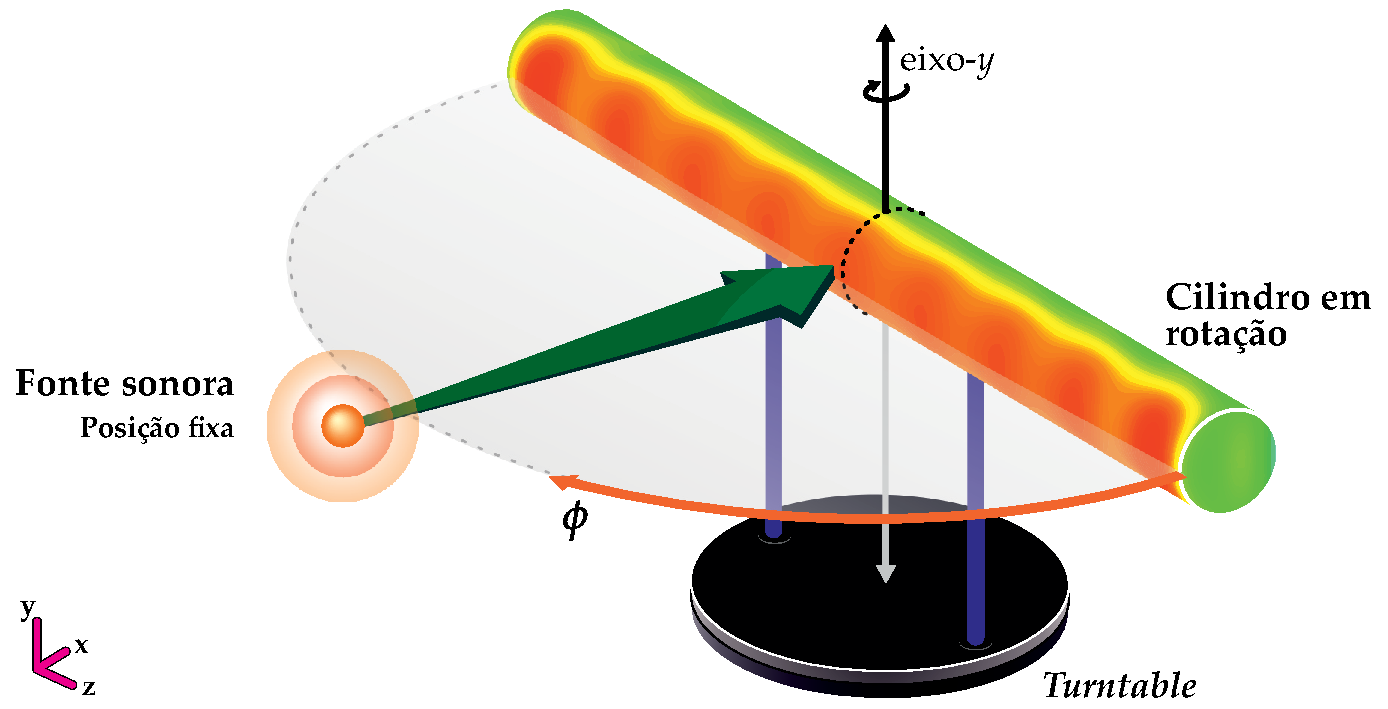
\includegraphics[width=0.85\linewidth]{figuras/Measurement-Scheme-Fonseca-2013.pdf}%
	\caption{Medição de beamforming com arranjo cilíndrico (adaptado de Fonseca \cite{Fonseca-2013}).}%
	\label{fig:beamforming}%
\end{figure}

\begin{figure}[!ht]
    \centering
    \begin{minipage}[t]{.48\textwidth}
        \centering
        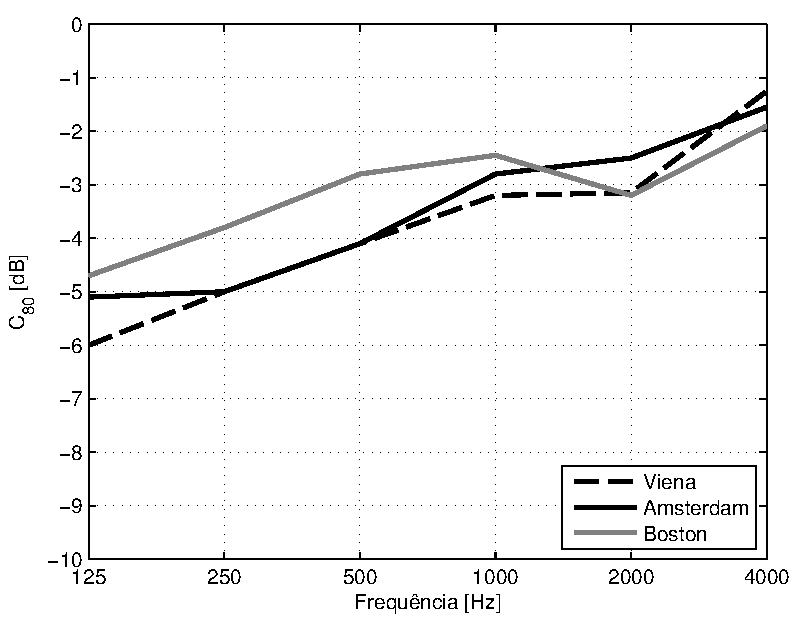
\includegraphics[width=1\linewidth,page=1]{figuras/C80_Concerthalls-Brandao-2017.pdf}
        \caption{Efeitos de interferência em salas\\ (\textit{comb filtering}). Fonte: Brandão, 2017 \cite{Brandao-2017}.
}
        \label{fig:ladoE}
    \end{minipage}%
		\quad
    \begin{minipage}[t]{0.48\textwidth}
        \centering
        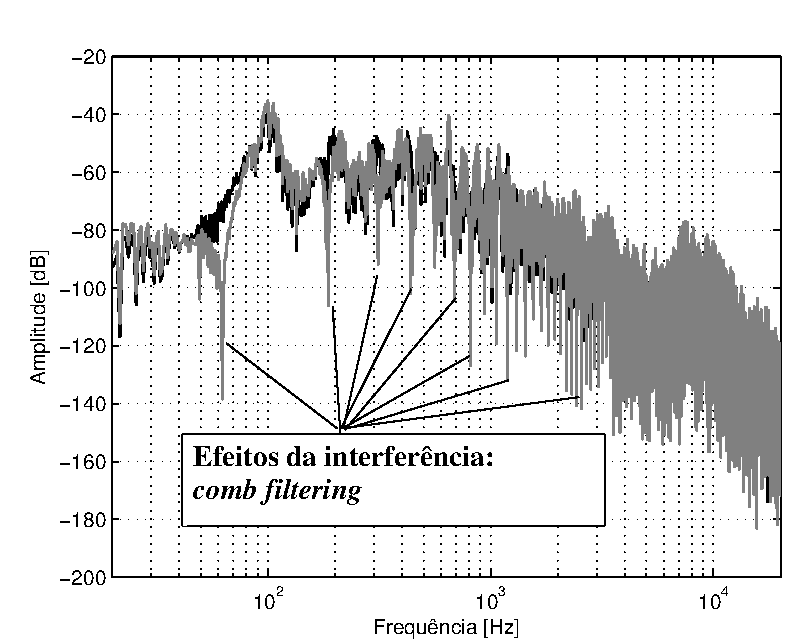
\includegraphics[width=1\linewidth,page=1]{figuras/Combfilter-Brandao-2017.pdf}
        \caption{C$_{80}$ para salas distintas. As figuras podem ser colocadas lado a lado (retirado de Brandão \cite{Brandao-2017}).}
        \label{fig:ladoD}
    \end{minipage}
\end{figure}

%\pagebreak
%\clearpage
\hspace{\baselineskip}

Recomenda-se que gráficos, figuras, fotos e qualquer arquivo gráfico, estejam inseridos no texto em formato jpg e/ou png com boa qualidade (ou ainda em formato pdf para o \LaTeX\xspace). Atente para que os elementos de gráficos e figuras sejam legíveis (sobretudo se a informação for pertinente).

%%%%%%%%%%%%%%%%%%%%%%%%%%%%%%%%%%%%%%%%%%%%%%%%%%%%%%%%%%%%%%%%%%%%%%%%%%%%%%%%%%%%%%%%%%%%%%%%%%%%%%%%
\section{Organização do trabalho}

A estrutura do artigo deverá conter pelo menos os seguintes itens:
%
\begin{itemize} \itemsep=5pt
	\item Introdução: visão geral sobre o assunto com definição dos objetivos do trabalho, indicando a sua relevância;
	\item Desenvolvimento: como o trabalho foi realizado;
	\item Resultados e discussões: parciais ou conclusivos, conforme a modalidade do trabalho (graduação, pós-graduação, tecnológico ou profissional), fazendo referência a medidas e cálculos estatísticos aplicados, se for o caso;
	\item Conclusões ou Considerações finais: basear-se nos dados apresentados no item Resultados e discussões, referindo-se aos objetivos do trabalho;
	\item Agradecimentos (quando existe financiamento, ou seja pertinente); e
	\item Referências: apresentar bibliografia utilizada.
\end{itemize}
%
Outros elementos pós-textuais como apêndices e anexos são opcionais, desde que não excedam o limite de páginas estabelecido. 

Para a confecção das referências deve-se utilizar a norma brasileira. As referências devem ser numeradas conforme ordem de aparição, utilizando colchetes \cite{Gomes-2015} (conforme a norma brasileira permite). Toda referência deve ser citada durante o texto. As referências devem estar em tamanho 10~pts com espaçamento simples. As referências \cite{Mareze-2017,Fonseca-2013,Brandao-2017,Gomes-2015,Oppenheim-2010,Muller-2001,Borges-2018} deste modelo de artigo são apenas ilustrativas (para efeito de compreensão). 

Recomenda-se evitar a apresentação de referências em notas de rodapé. As referências devem ser citadas no texto do artigo, ao final, usando o último sobrenome do autor e o ano de publicação, o qual deve estar entre parênteses (conforme normas vigentes). Dependendo do contexto, o nome do autor pode ou não ser escrito, conforme o exemplo a seguir: 
%
\begin{itemize} \itemsep=2pt
	\item 	``... Mareze et al. \cite{Mareze-2017} trabalharam com medições em tubo de impedância...'' ou 
	\item ``... para o estudo de acústica de salas \cite{Brandao-2017} recomenda-se a leitura de um livro texto...'' ou
	\item ``... aplicando a Transformada de Fourier nos sinais de entrada \cite{Oppenheim-2010}. '' ou ainda
	\item ``... Fonseca \cite{Fonseca-2013} aclarou que o \textit{beamforming} é uma técnica de imageamento acústico.''
\end{itemize}
%
Todas as referências da lista de referências devem ser citadas no texto, a tipografia deverá ser escrita com corpo 10 pts.  

Em referências com até três autores, por exemplo, Müller e Massarani \cite{Muller-2001}, ambos devem ser citados (quando evocados). No caso de mais de três autores, por exemplo, Gomes \etal \cite{Gomes-2015,Mareze-2017,Borges-2018} deve-se citar somente o último nome do primeiro autor seguido da expressão ``\etal''. Ainda, ao citar mais de uma referência, utilize apenas um colchete, veja alguns exemplos a seguir:
%
\begin{itemize} \itemsep=2pt
	\item 	``Trabalhos em temas de acústica e vibrações \cite{Mareze-2017,Fonseca-2013,Brandao-2017}.''
	\item ``Trabalhos em temas de acústica \cite{Mareze-2017,Oppenheim-2010,Muller-2001,Borges-2018}.''
	\item ``Trabalhos com análise estatística \cite{Mareze-2017, Brandao-2017, Borges-2018}.''
	\item ``Trabalhos com análise dinâmica [\citenum{Mareze-2017}, \citenum{Fonseca-2013}, \citenum{Brandao-2017}].''
\end{itemize}

É responsabilidade dos autores a preparação e envio dos artigos em seu formato final. Por este motivo, alertamos que verifiquem com atenção a formatação de seus artigos, especialmente gráficos e fotos, quanto à legibilidade e qualidade para impressão. Os artigos deverão ser enviados (submetidos) no formato DOCX e PDF, podendo ser desenvolvidos em Ms Word (ou similar) ou em \LaTeX\xspace. Os arquivos que deverão ser enviados:
%
\begin{itemize} \itemsep=2pt
	\item ``.pdf'' e ``.docx'' para usuários de Ms Word (ou similar) e
	\item ``.pdf'' e ``.zip'' contendo os arquivos fonte para usuários de \LaTeX\xspace,
\end{itemize}
%
sendo que o tamanho do arquivo PDF não ultrapasse 12 megabytes. Em caso de dúvidas, entre em contato com a comissão do evento.


%%%%%%%%%%%%%%%%%%%%%%%%%%%%%%%%%%%%%%%%%%%%%%%%%%%%%%%%%%%%%%%%%%%%%%%%%%%%%%%%%%%%%%%%%%%%%%%%%%%%%%%%
\section{Agradecimentos}

Os autores gostariam de agradecer ao financiamento do CNPq, por exemplo.

%%%%%%%%%%%%%%%%%%%%%%%%%%%%%%%%%%%%%%%%%%%%%%%%%%%%%%%%%%%%%%%%%%%%%%%%%%%%%%%%%%%%%%%%%%%%%%%%%%%%%%%%
%%%%%%%%%%%%%%%%%%%%%%%%%%%%%%%%%%%%%%%%%%%%%%%%%%%%%%%%%%%%%%%%%%%%%%%%%%%%%%%%%%%%%%%%%%%%%%%%%%%%%%%%
\renewcommand{\refname}{\uppercase{Referências}} \addcontentsline{toc}{section}{\refname}% 
\bibliographystyle{unsrtnat-br}
{\fontsize{10}{12}\selectfont  

%%%%%%%%%%%%%%%%%%%%%%%%%%%%%%%%%%%%%%%%%%%%%%%%%%%%%%%%%%%%%%%%%%%%%%%%%
%%% Método 1
% Referências são chamadas de um arquivo contendo todas as referências
% Neste caso, dentro do arquivo bibliografia, este arquivo pode ser criado 
% e editado com JabRef, por exemplo
\bibliography{bibliografia}

%%%%%%%%%%%%%%%%%%%%%%%%%%%%%%%%%%%%%%%%%%%%%%%%%%%%%%%%%%%%%%%%%%%%%%%%%
%%% Método 2
% Referências direto no arquivo, porém a escrita, as configurações
%e o reordenamento são manuais

%%% Escreva a referências dentro desse ambiente
%\begin{thebibliography}{20}
%
%\bibitem{Mareze-2017}
%Mareze, P. H.; Copetti, G.; Brandão, E.; Fonseca, D'A. W.; Dresch, F. e Specht, L. P. Modelagem da absorção acústica de camadas porosas asfálticas. In: \textit{XXVIII Encontro da Sociedade Brasileira de Acústica}, Sobrac~2017, Brasília, DF, 2017.
%
%\bibitem{Fonseca-2013}
%Fonseca, D’A. W. Beamforming considerando difração acústica em superfícies cilíndricas. 2013. Tese de doutorado. Universidade Federal de Santa Catarina, Florianópolis, SC.
%
%\bibitem{Brandao-2017}
%Brandão, E. Acústica de Salas: Projeto e Modelagem. 1ª ed. São Paulo: Blucher, 2016.
%
%\bibitem{Gomes-2015}
%Gomes, M. H. A.; Bonifacio, P. R. O.; Carvalho, M. O. M. e Azikri de Deus, H. P. A Vibro Acoustic Method for Non Destructive Test of Composite Sandwich Structures. Applied Mechanics and Materials, v. 751, p. 153-158, 2015.
%
%\bibitem{Oppenheim-2010}
%Oppenheim, A. e Willsky, A. S. Sinais e Sistemas. 2ª ed. São Paulo: Pearson, 2010.
%
%\bibitem{Muller-2001}
%Müller, S. e Massarani, P. Transfer-function measurement with sweeps. Journal of the Audio Engineering Society, v. 49, n. 6, p. 443–471, 2001.
%
%\bibitem{Borges-2018}
%Borges, J.; Pacheco, F.; Tutikian, B. e de Oliveira M. An experimental study on the use of waste aggregate for acoustic attenuation: EVA and rice husk composites for impact noise reduction. Construction and Building Materials, v. 161, p. 501-508, 2018.
%
%\end{thebibliography}
}
%%%%%%%%%%%%%%%%%%%%%%%%%%%%%%%%%%%%%%%%%%%%%%%%%%%%%%%%%%%%%%%%%%%%%%%%%%%%%%%%%%%%%%%%%%%%%%%%%%%%%%%%
%%%%%%%%%%%%%%%%%%%%%%%%%%%%%%%%%%%%%%%%%%%%%%%%%%%%%%%%%%%%%%%%%%%%%%%%%%%%%%%%%%%%%%%%%%%%%%%%%%%%%%%%
\appendix
\section{Apêndice - Comandos adicionais e exemplos para \LaTeX}

Há incluído nesta distribuição uma série de comandos adicionais (e opcionais) dentro do pacote {\ttfamily Will.sty}, desenvolvidos pelo Prof. William D'Andrea Fonseca (Eng. Acústica -- UFSM). Eles facilitarão a escrita em \LaTeX\xspace, alguns deles são mostrados aqui. Todavia, recomenda-se que o pacote seja aberto e lido. Veja neste documento os códigos que geram os exemplos a seguir:
%
\vspace{-5pt}
\begin{itemize} \itemsep=2pt
	\item Temperatuda de 30\dg C.
	\item A \subfigura{fig.figA} mostra...
	\item A \figura{fig.subfig} contém duas subfiguras.
	\item \eg, \ie, \etc, \etal 
	\item Raiz quadrada fechada $\sqrt{1982}$ ou aberta $\oldsqrt{1982}$.
	\item Texto em pé no ambiente matemático ($\tx{AB}_i$), subscrito ($T\txu{Sabine}$) ou sobrescrito ($C\txup{asa}$).
	\item Convenções matemáticas e/ou operadores: $\ji \dt \e \xp$ escritas em pé.
	\item $\F$ de Fourier.
	\item Entre outros...
\end{itemize}


\begin{figure}[H]
  \centering
	\subfloat[Figura do lado esquerdo]{\label{fig.figA}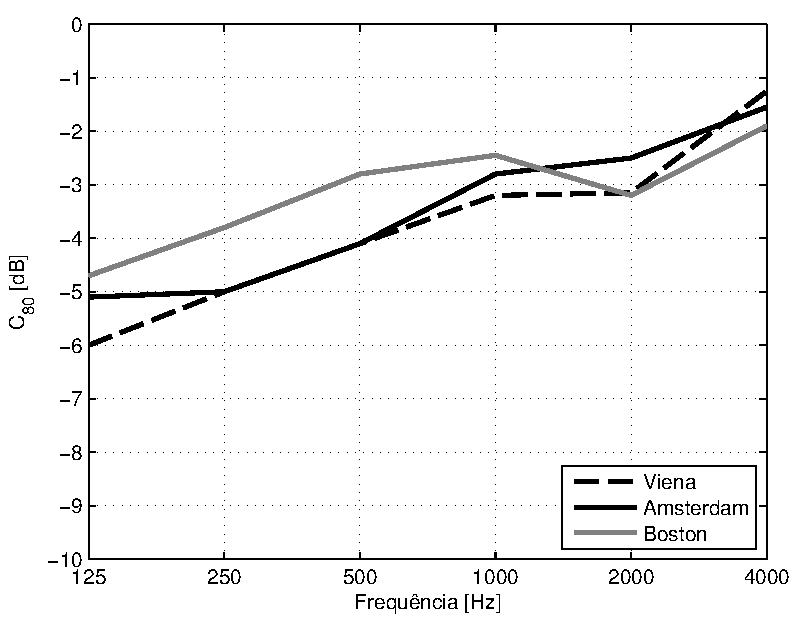
\includegraphics[width=0.48\linewidth,page=1]{figuras/C80_Concerthalls-Brandao-2017.pdf}}
	\quad
  \subfloat[Figura do lado esquerdo]{\label{fig.figB}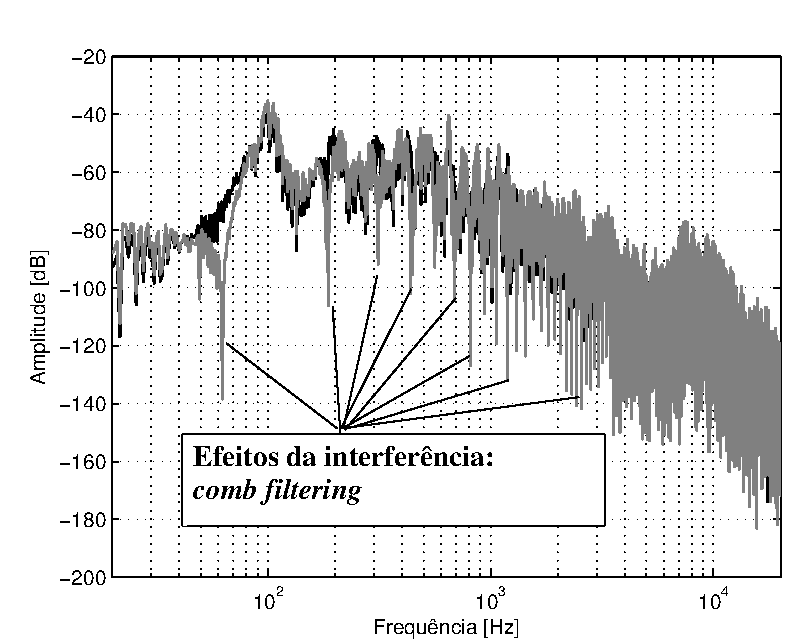
\includegraphics[width=0.48\linewidth,page=1]{figuras/Combfilter-Brandao-2017.pdf}}	

  \caption{Exemplo de figura com duas figuras, uma de cada lado.}
  \label{fig.subfig}
\end{figure}

%%%%%%%%%%%%%%%%%%%%%%%%%%%%%%%%%%%%%%%%%%%%%%%%%%%%%%%%%%%%%%%%%%%%%%%%%%%%%%%%%%%%%%%%%%%%%%%%%%%%%%%%
%%%%%%%%%%%%%%%%%%%%%%%%%%%%%%%%%%%%%%%%%%%%%%%%%%%%%%%%%%%%%%%%%%%%%%%%%%%%%%%%%%%%%%%%%%%%%%%%%%%%%%%%
\end{document}
%%%%%%%%%%%%%%%%%%%%%%%%%%%%%%%%%%%%%%%%%%%%%%%%%%%%%%%%%%%%%%%%%%%%%%%%%%%%%%%%%%%%%%%%%%%%%%%%%%%%%%%%
% EOF

